\documentclass[11pt,dvipdfmx]{jarticle}

\usepackage{eee}
\usepackage{subfig}
\usepackage{graphicx}
\usepackage{pdfpages}
\usepackage{float}
\usepackage{amsmath}
\usepackage{amssymb}
\usepackage{color}
\usepackage{multirow}
\usepackage{adjustbox}
\usepackage{url}
\usepackage{mymacros}
\usepackage{here}

\begin{document}

%表紙%
%%%%%%%%%%%%%%%%%%%%%%%%%%%%%%%%%%%%%%%%%%%%%
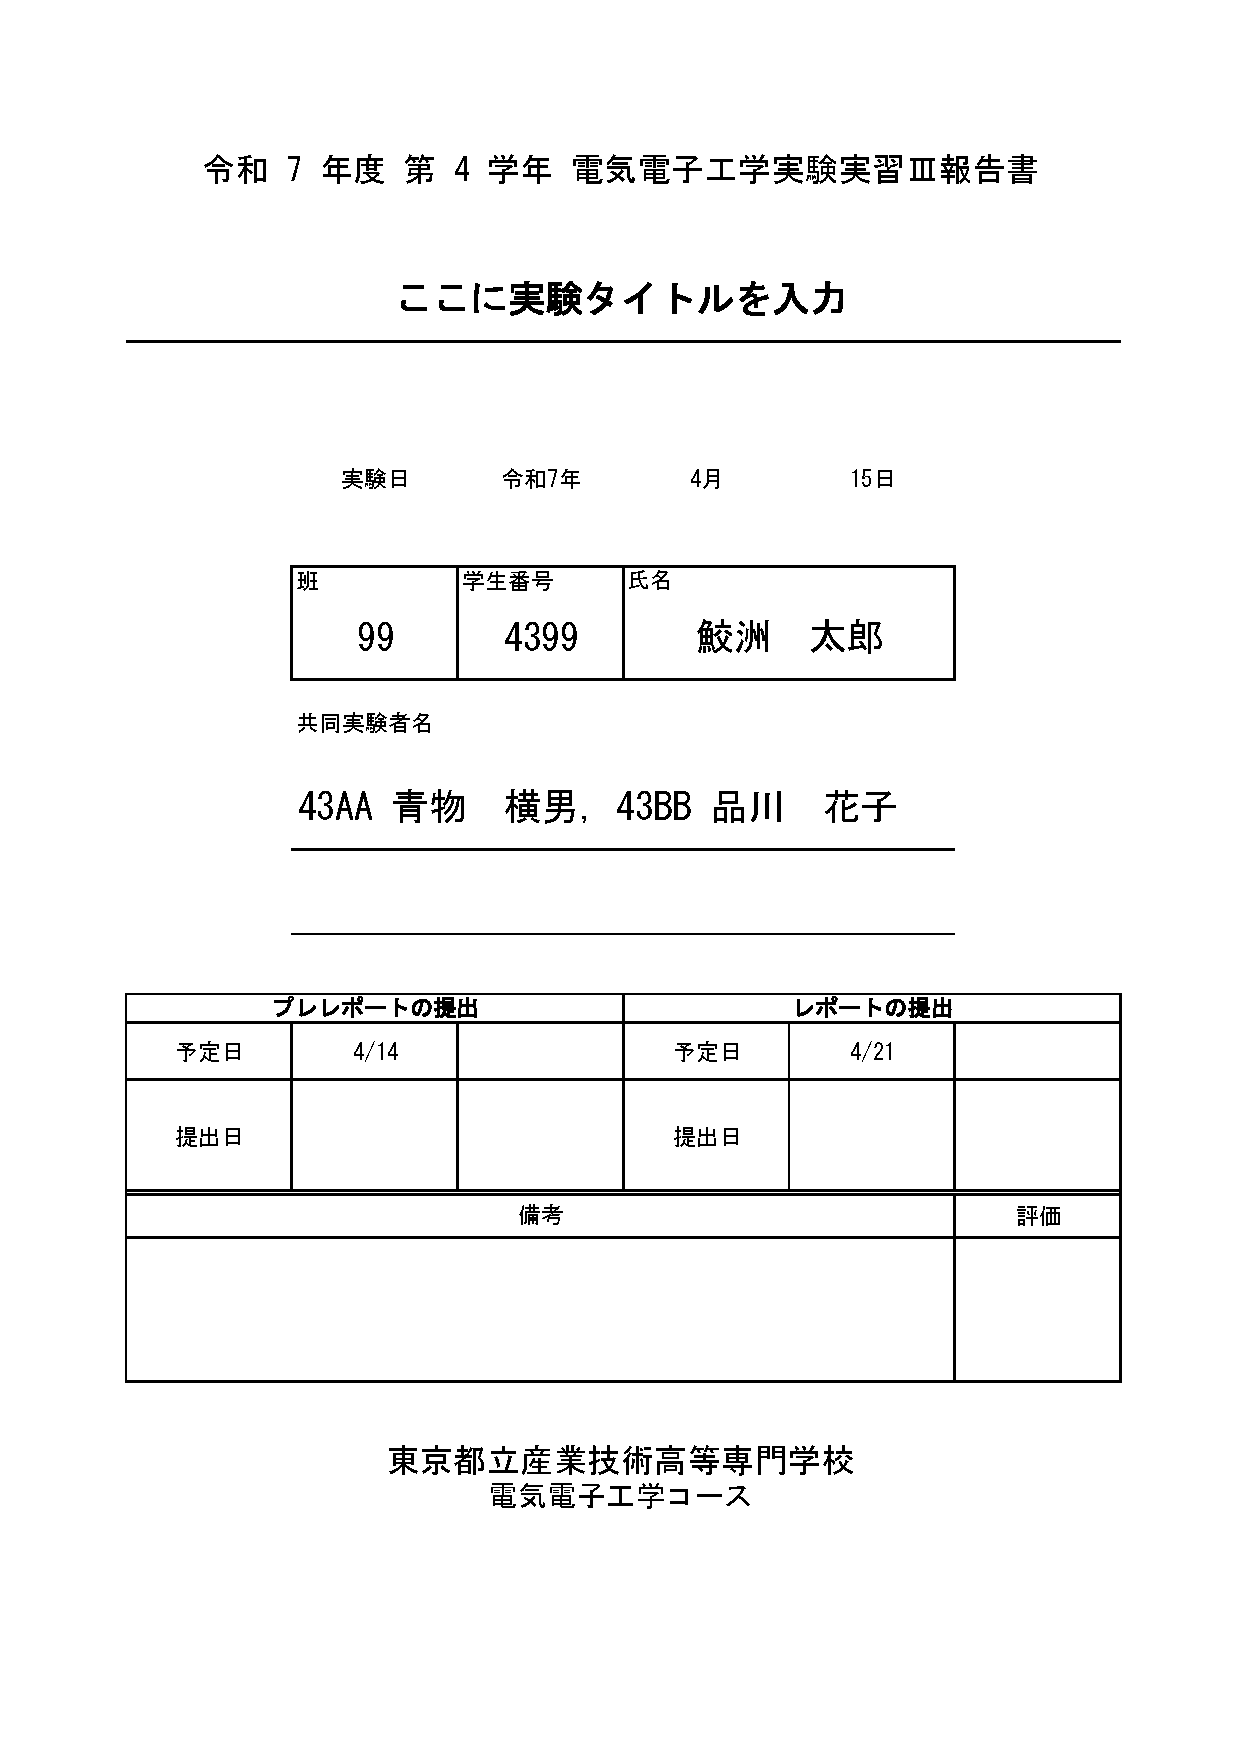
\includepdf[noautoscale=true]{Title.pdf}
%%%%%%%%%%%%%%%%%%%%%%%%%%%%%↑↑ここのファイル名を表紙PDFファイル名に変更

\section{目的}
本実験の目的は、時間信号と周波数スペクトルの相互関係を理解するとともに、アナログフィルタを用いた周波数選択によって時間信号が変化する様子を理解することである。

\section{原理}

\subsection{フーリエ級数}
周期 $T$ の周期関数 $f(t)$ は、以下のような三角関数の級数で表される:
\begin{align}
f(t) = a_0 + \sum_{n=1}^{\infty} a_n \cos \frac{2\pi nt}{T} + \sum_{n=1}^{\infty} b_n \sin \frac{2\pi nt}{T}
\end{align}

各係数は以下のように求められる:
\begin{align}
a_0 &= \frac{1}{T} \int_{-T/2}^{T/2} f(t) dt \\
a_n &= \frac{2}{T} \int_{-T/2}^{T/2} f(t) \cos \frac{2\pi nt}{T} dt \\
b_n &= \frac{2}{T} \int_{-T/2}^{T/2} f(t) \sin \frac{2\pi nt}{T} dt
\end{align}

\subsection{伝達関数とRCフィルタ}
線形システムの動作は伝達関数によって記述され、周波数 $f_n$ に対して次のように定義される:
\begin{align}
H(f_n) = |H(f_n)| e^{j\theta(f_n)}
\end{align}

RC低域通過フィルタ(LPF)の伝達関数は、
\begin{align}
H(f) = \frac{1}{1 + j\frac{f}{f_1}}
\end{align}
ただし、$f_1 = \frac{1}{2\pi RC}$ は遮断周波数である。

RC高域通過フィルタ(HPF)の伝達関数は、
\begin{align}
H(f) = \frac{1}{1 + j\frac{f_2}{f}}
\end{align}
ただし、$f_2 = \frac{1}{2\pi RC}$ である。

\subsection{離散フーリエ変換(DFT)}
時間領域の離散信号 $f_n$ に対して、離散フーリエ変換は以下の式で与えられる:
\begin{align}
F_k = \sum_{n=0}^{N-1} f_n e^{-j \frac{2\pi kn}{N}}
\end{align}

\section{実験方法}

\subsection{時間信号の測定}
VirtualBenchを用いて、以下の手順で時間信号を測定した:

\begin{enumerate}
  \item \wfig{実験回路1}に示すとおりに結線した。
  \item DUTとして\wtab{各種LCフィルタ}に示すLPFを接続した。
  \item FGENで正弦波を選択し、$10\,\mathrm{kHz}$から$1\,\mathrm{MHz}$までの周波数、および遮断周波数における入力・出力波形を測定し、数値データとして保存した。
  \item 各班員が用意した任意波形、および班で用意したガウシアンパルスをFGENに設定し、それぞれ測定を行い、数値データとして保存した。
  \item DUTを\wtab{各種LCフィルタ}に示すHPF, BPF, BEFへ変更し、同様の手順で測定を繰り返した。
  \item 測定結果から、各周波数における振幅比(dB)および位相差を計算し、グラフを作成した。
  \item 任意波形およびガウシアンパルスについては、入力信号と出力信号を同一グラフにプロットし、波形の変化を確認できるようにした。
\end{enumerate}
\begin{figure}[H]
  \centering
  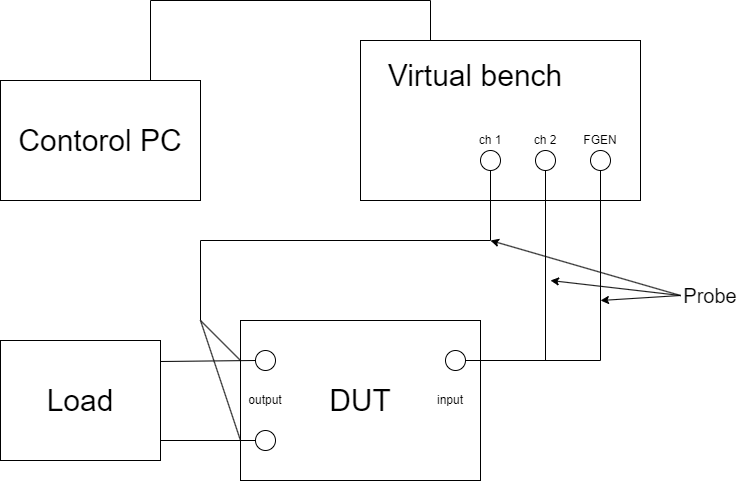
\includegraphics[width=0.8\textwidth]{fig/VirtualBench.drawio.png}
  \caption{時間信号測定用の実験回路}
  \label{fig:実験回路1}  
\end{figure}
\begin{table}[H]
  \centering
  \caption{各種LCフィルタ}
  \label{tab:各種LCフィルタ}
  \begin{tabular}{|c|m{0.22\textwidth}|c|}
    \hline
    フィルタの種類 & 回路図 & 素子値の計算 $f_c$ \\
    \hline
    LPF & 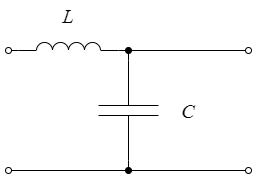
\includegraphics[width=0.2\textwidth]{fig/LPF.drawio.png} & $f_c = 150\,\mathrm{kHz}$ \\
    \hline
    HPF & 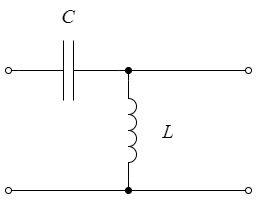
\includegraphics[width=0.2\textwidth]{fig/HPF.drawio.png} & $f_c = 140\,\mathrm{kHz}$ \\
    \hline
    BPF & 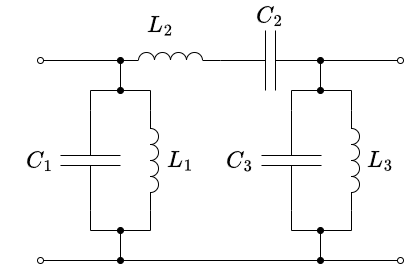
\includegraphics[width=0.2\textwidth]{fig/BPF.drawio.png} & $f_{c1} = 50\,$kHz,$f_{c2} = 200\,$kHz \\
    \hline
    BEF & 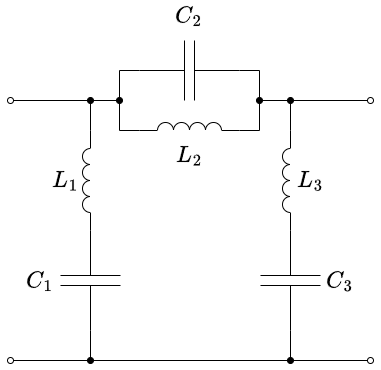
\includegraphics[width=0.2\textwidth]{fig/BEF.drawio.png} & $f_{c1} = 100\,$kHz,$f_{c2} = 140\,$kHz \\
    \hline
  \end{tabular}
\end{table}
\subsection{周波数特性の測定}
NanoVNAを用いてフィルタの周波数特性を測定した。以下の手順で実施した:

\begin{enumerate}
  \item \wfig{実験回路2}に示すとおりに結線した。
  \item ポートをCOM3に設定し、測定周波数範囲を$50\,\mathrm{kHz}$から$1\,\mathrm{MHz}$に設定した。
  \item キャリブレーション(open, short, load, isolation, through)を行い、「save0」に記録した。
  \item DUTとして各フィルタ(LPF, HPF, BPF, BEF)を接続し、測定データを「s2p」形式で保存した。
\end{enumerate}
\begin{figure}[H]
  \centering
  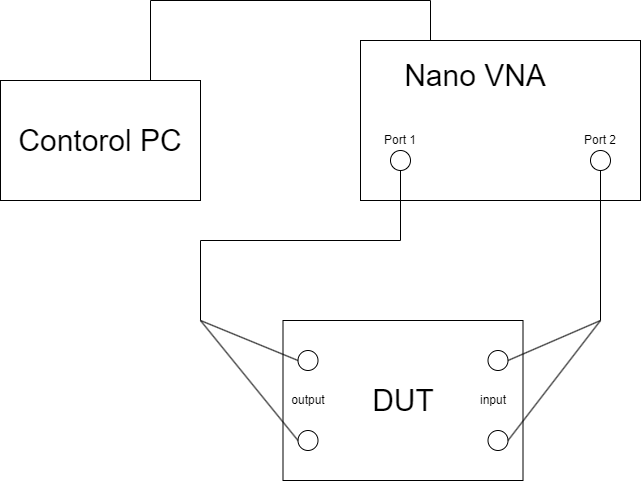
\includegraphics[width=0.8\textwidth]{fig/VNA.drawio.png}
  \caption{周波数特性測定用の実験回路}
  \label{fig:実験回路2}
\end{figure}

\section{実験結果}
<<<<<<< HEAD
\subsection{時間信号の測定結果}

\subsubsection{2段LPFの測定結果}

\begin{figure}[H]
  \centering
  \includegraphics[width=0.8\textwidth]{graphs/10kHz_LPF_characteristic.png}
  \caption{LPFの10 kHzの場合の入力・出力波形}
  \label{fig:LPF_10kHz}
\end{figure}
\begin{figure}[H]
  \centering
  \includegraphics[width=0.8\textwidth]{graphs/20kHz_LPF_characteristic.png}
  \caption{LPFの20 kHzの場合の入力・出力波形}
  \label{fig:LPF_20kHz}
\end{figure}

\begin{figure}[H]
  \centering
  \includegraphics[width=0.8\textwidth]{graphs/40kHz_LPF_characteristic.png}
  \caption{LPFの40 kHzの場合の入力・出力波形}
  \label{fig:LPF_40kHz}
\end{figure}

\begin{figure}[H]
  \centering
  \includegraphics[width=0.8\textwidth]{graphs/50kHz_LPF_characteristic.png}
  \caption{LPFの50 kHzの場合の入力・出力波形}
  \label{fig:LPF_50kHz}
\end{figure}

\begin{figure}[H]
  \centering
  \includegraphics[width=0.8\textwidth]{graphs/80kHz_LPF_characteristic.png}
  \caption{LPFの80 kHzの場合の入力・出力波形}
  \label{fig:LPF_80kHz}
\end{figure}

\begin{figure}[H]
  \centering
  \includegraphics[width=0.8\textwidth]{graphs/100kHz_LPF_characteristic.png}
  \caption{LPFの100 kHzの場合の入力・出力波形}
  \label{fig:LPF_100kHz}
\end{figure}

\begin{figure}[H]
  \centering
  \includegraphics[width=0.8\textwidth]{graphs/200kHz_LPF_characteristic.png}
  \caption{LPFの200 kHzの場合の入力・出力波形}
  \label{fig:LPF_200kHz}
\end{figure}

\begin{figure}[H]
  \centering
  \includegraphics[width=0.8\textwidth]{graphs/400kHz_LPF_characteristic.png}
  \caption{LPFの400 kHzの場合の入力・出力波形}
  \label{fig:LPF_400kHz}
\end{figure}

\begin{figure}[H]
  \centering
  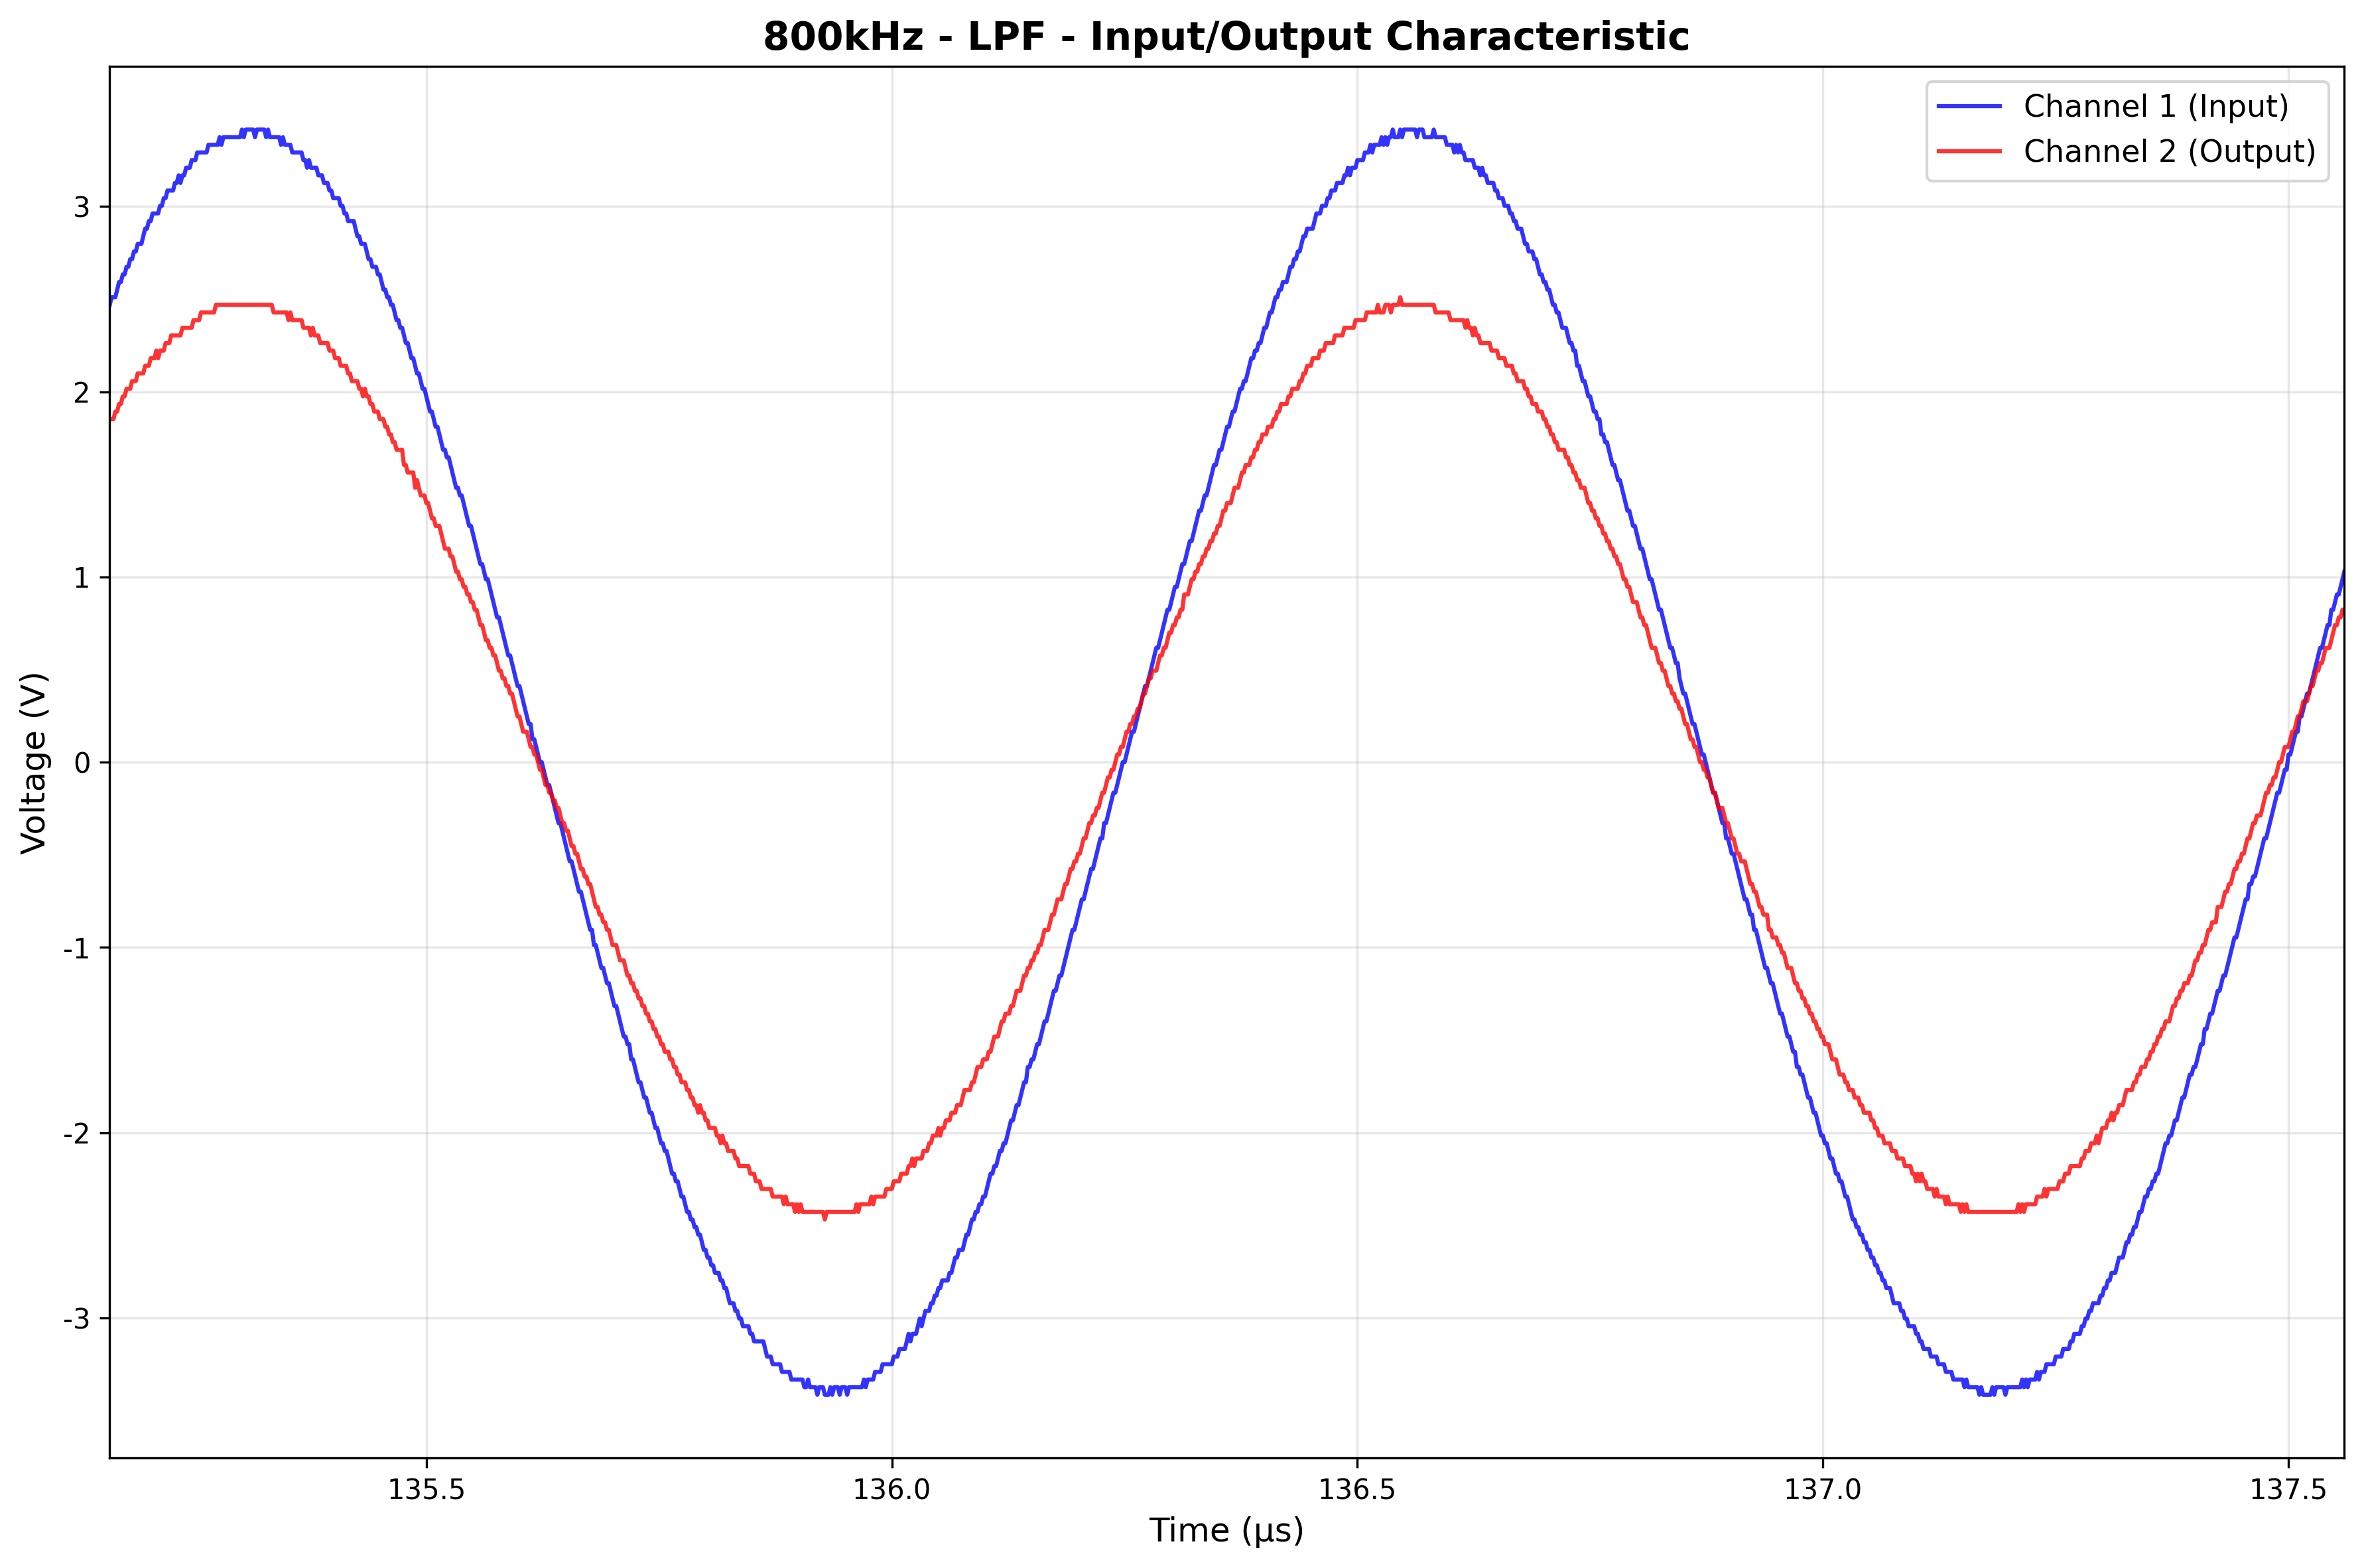
\includegraphics[width=0.8\textwidth]{graphs/800kHz_LPF_characteristic.png}
  \caption{LPFの800 kHzの場合の入力・出力波形}
  \label{fig:LPF_800kHz}
\end{figure}

\begin{figure}[H]
  \centering
  \includegraphics[width=0.8\textwidth]{graphs/1000kHz_LPF_characteristic.png}
  \caption{LPFの1000 kHzの場合の入力・出力波形}
  \label{fig:LPF_1000kHz}
\end{figure}







=======
\subsection{時間信号の特性}
\subsubsection{LPF}
LPFの入力・出力波形を以下に示す。LPFでは、入力信号と出力信号の波形がどのように変化するかを確認した。

% LPF関連グラフ
\begin{figure}[H]
  \centering
  \includegraphics[width=0.8\textwidth]{fig/10kHz_LPF_characteristic.png}
  \caption{10kHz LPF波形}
\end{figure}
\begin{figure}[H]
  \centering
  \includegraphics[width=0.8\textwidth]{fig/20kHz_LPF_characteristic.png}
  \caption{20kHz LPF波形}
\end{figure}
\begin{figure}[H]
  \centering
  \includegraphics[width=0.8\textwidth]{fig/40kHz_LPF_characteristic.png}
  \caption{40kHz LPF波形}
\end{figure}
\begin{figure}[H]
  \centering
  \includegraphics[width=0.8\textwidth]{fig/50kHz_LPF_characteristic.png}
  \caption{50kHz LPF波形}
\end{figure}
\begin{figure}[H]
  \centering
  \includegraphics[width=0.8\textwidth]{fig/80kHz_LPF_characteristic.png}
  \caption{80kHz LPF波形}
\end{figure}
\begin{figure}[H]
  \centering
  \includegraphics[width=0.8\textwidth]{fig/100kHz_LPF_characteristic.png}
  \caption{100kHz LPF波形}
\end{figure}
\begin{figure}[H]
  \centering
  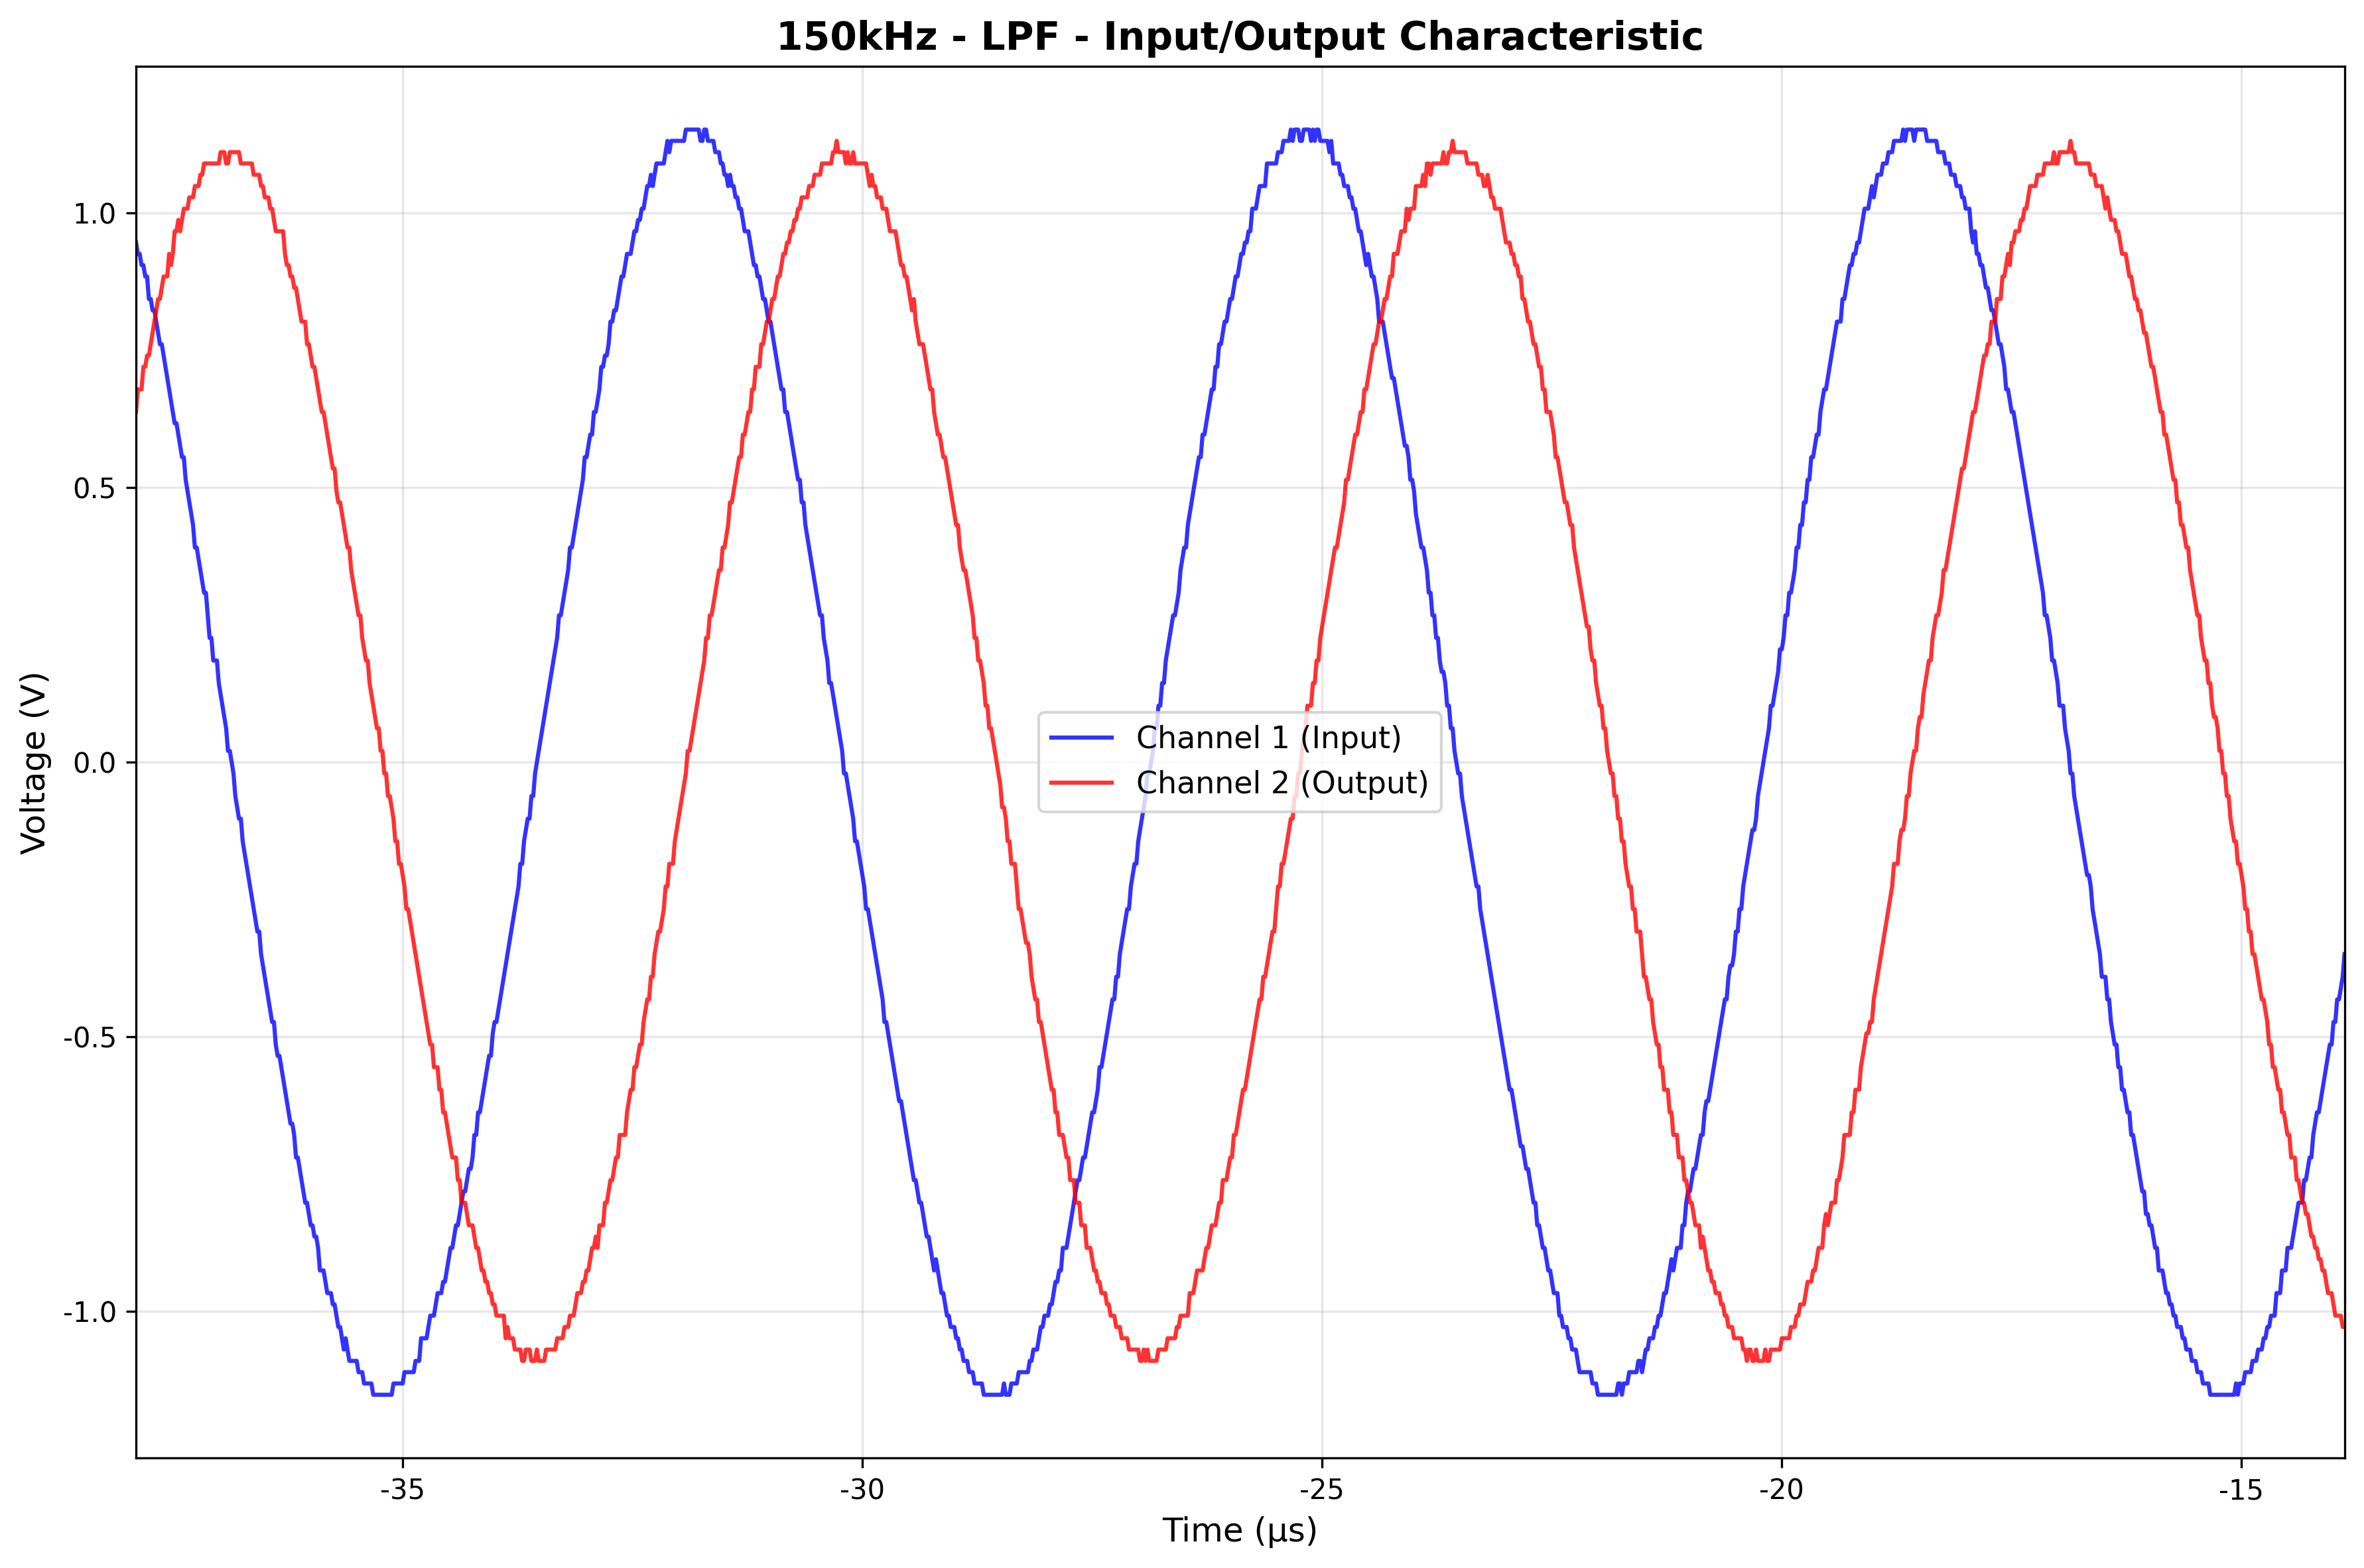
\includegraphics[width=0.8\textwidth]{fig/150kHz_LPF_characteristic.png}
  \caption{150kHz LPF波形}
\end{figure}
\begin{figure}[H]
  \centering
  \includegraphics[width=0.8\textwidth]{fig/200kHz_LPF_characteristic.png}
  \caption{200kHz LPF波形}
\end{figure}
\begin{figure}[H]
  \centering
  \includegraphics[width=0.8\textwidth]{fig/400kHz_LPF_characteristic.png}
  \caption{400kHz LPF波形}
\end{figure}
\begin{figure}[H]
  \centering
  \includegraphics[width=0.8\textwidth]{fig/1000kHz_LPF_characteristic.png}
  \caption{1000kHz LPF波形}
\end{figure}
\begin{figure}[H]
  \centering
  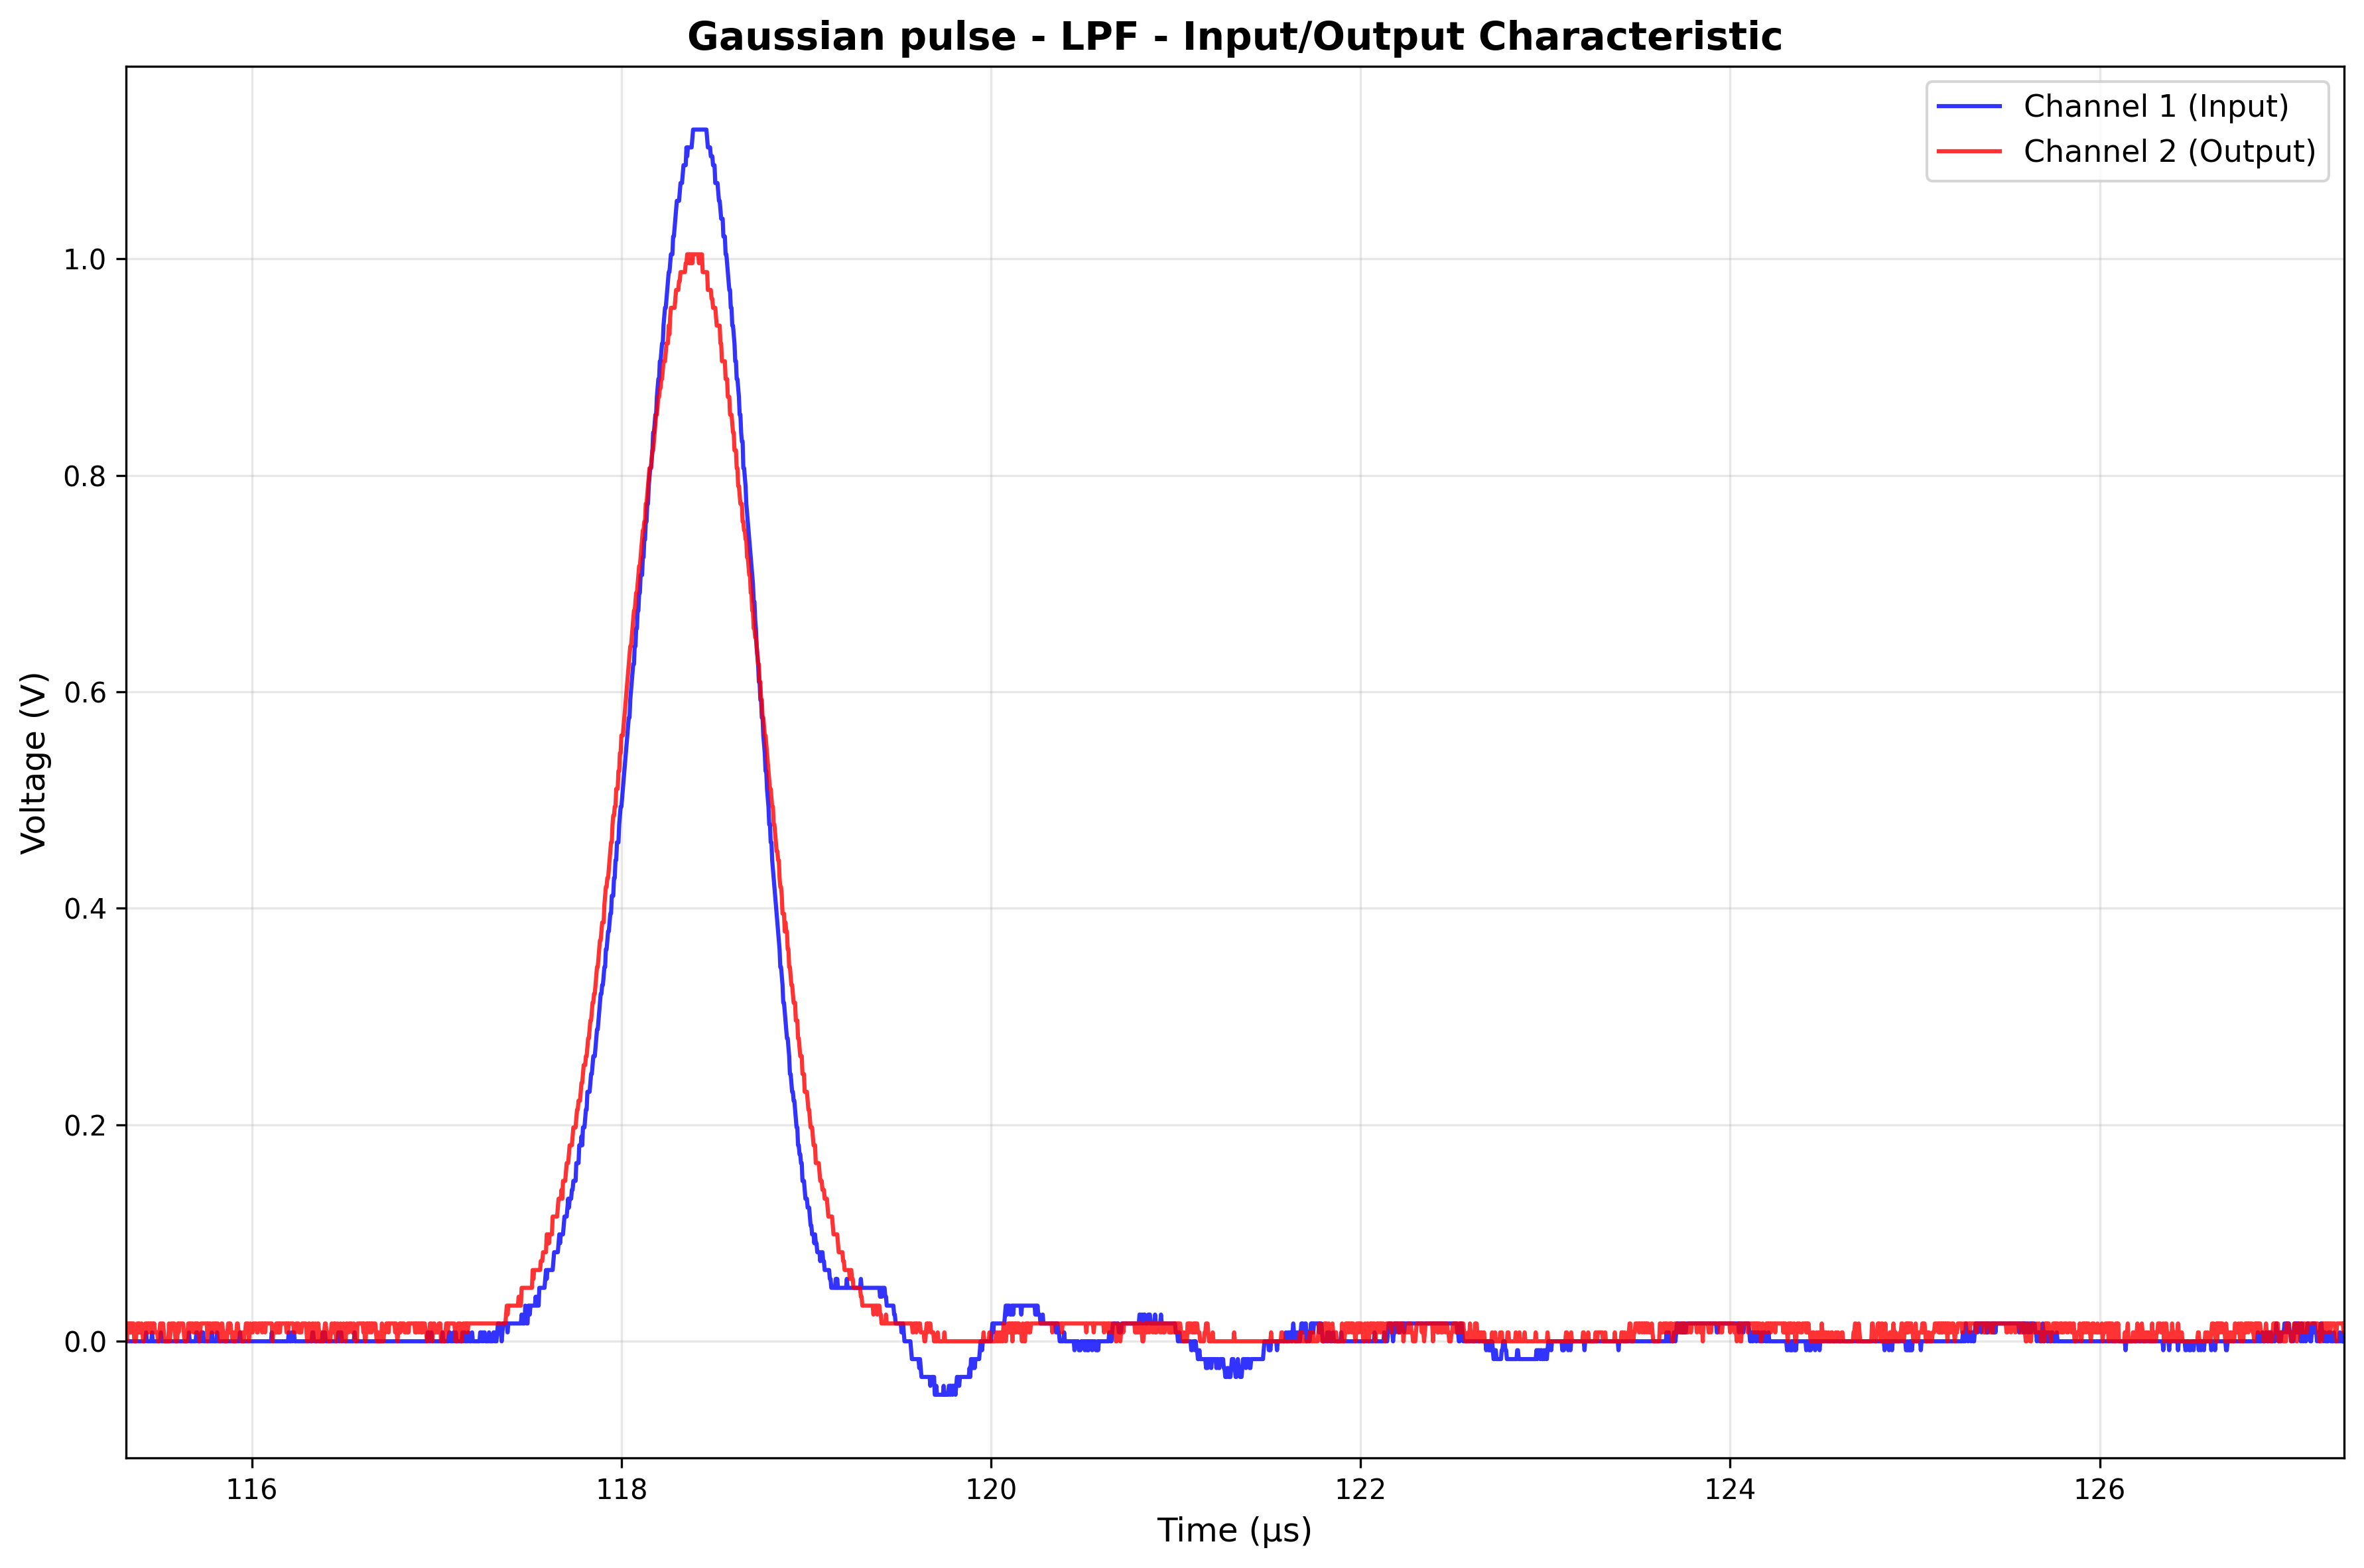
\includegraphics[width=0.8\textwidth]{fig/Gaussian_pulse_LPF_characteristic.png}
  \caption{Gaussian pulse LPF波形}
\end{figure}
\begin{figure}[H]
  \centering
  \includegraphics[width=0.8\textwidth]{fig/Original_wave1_LPF_characteristic.png}
  \caption{Original wave1 LPF波形}
\end{figure}
\begin{figure}[H]
  \centering
  \includegraphics[width=0.8\textwidth]{fig/Original_wave2_LPF_characteristic.png}
  \caption{Original wave2 LPF波形}
\end{figure}
\begin{figure}[H]
  \centering
  \includegraphics[width=0.8\textwidth]{fig/Original_wave3_LPF_characteristic.png}
  \caption{Original wave3 LPF波形}
\end{figure}
\begin{figure}[H]
  \centering
  \includegraphics[width=0.8\textwidth]{fig/Original_wave4_LPF_characteristic.png}
  \caption{Original wave4 LPF波形}
\end{figure}

\section{考察}
お

\section{結論}
か

\section{謝辞}
き


\begin{thebibliography}{99}
\bibitem{1} 古川 浩洋,""高専男子学生の体格と運動能力に関する研究"",論文集「高専教育」,p. 151-158,1998.
\end{thebibliography}

\end{document}